\documentclass[1p]{elsarticle_modified}
%\bibliographystyle{elsarticle-num}

%\usepackage[colorlinks]{hyperref}
%\usepackage{abbrmath_seonhwa} %\Abb, \Ascr, \Acal ,\Abf, \Afrak
\usepackage{amsfonts}
\usepackage{amssymb}
\usepackage{amsmath}
\usepackage{amsthm}
\usepackage{scalefnt}
\usepackage{amsbsy}
\usepackage{kotex}
\usepackage{caption}
\usepackage{subfig}
\usepackage{color}
\usepackage{graphicx}
\usepackage{xcolor} %% white, black, red, green, blue, cyan, magenta, yellow
\usepackage{float}
\usepackage{setspace}
\usepackage{hyperref}

\usepackage{tikz}
\usetikzlibrary{arrows}

\usepackage{multirow}
\usepackage{array} % fixed length table
\usepackage{hhline}

%%%%%%%%%%%%%%%%%%%%%
\makeatletter
\renewcommand*\env@matrix[1][\arraystretch]{%
	\edef\arraystretch{#1}%
	\hskip -\arraycolsep
	\let\@ifnextchar\new@ifnextchar
	\array{*\c@MaxMatrixCols c}}
\makeatother %https://tex.stackexchange.com/questions/14071/how-can-i-increase-the-line-spacing-in-a-matrix
%%%%%%%%%%%%%%%

\usepackage[normalem]{ulem}

\newcommand{\msout}[1]{\ifmmode\text{\sout{\ensuremath{#1}}}\else\sout{#1}\fi}
%SOURCE: \msout is \stkout macro in https://tex.stackexchange.com/questions/20609/strikeout-in-math-mode

\newcommand{\cancel}[1]{
	\ifmmode
	{\color{red}\msout{#1}}
	\else
	{\color{red}\sout{#1}}
	\fi
}

\newcommand{\add}[1]{
	{\color{blue}\uwave{#1}}
}

\newcommand{\replace}[2]{
	\ifmmode
	{\color{red}\msout{#1}}{\color{blue}\uwave{#2}}
	\else
	{\color{red}\sout{#1}}{\color{blue}\uwave{#2}}
	\fi
}

\newcommand{\Sol}{\mathcal{S}} %segment
\newcommand{\D}{D} %diagram
\newcommand{\A}{\mathcal{A}} %arc


%%%%%%%%%%%%%%%%%%%%%%%%%%%%%5 test

\def\sl{\operatorname{\textup{SL}}(2,\Cbb)}
\def\psl{\operatorname{\textup{PSL}}(2,\Cbb)}
\def\quan{\mkern 1mu \triangleright \mkern 1mu}

\theoremstyle{definition}
\newtheorem{thm}{Theorem}[section]
\newtheorem{prop}[thm]{Proposition}
\newtheorem{lem}[thm]{Lemma}
\newtheorem{ques}[thm]{Question}
\newtheorem{cor}[thm]{Corollary}
\newtheorem{defn}[thm]{Definition}
\newtheorem{exam}[thm]{Example}
\newtheorem{rmk}[thm]{Remark}
\newtheorem{alg}[thm]{Algorithm}

\newcommand{\I}{\sqrt{-1}}
\begin{document}

%\begin{frontmatter}
%
%\title{Boundary parabolic representations of knots up to 8 crossings}
%
%%% Group authors per affiliation:
%\author{Yunhi Cho} 
%\address{Department of Mathematics, University of Seoul, Seoul, Korea}
%\ead{yhcho@uos.ac.kr}
%
%
%\author{Seonhwa Kim} %\fnref{s_kim}}
%\address{Center for Geometry and Physics, Institute for Basic Science, Pohang, 37673, Korea}
%\ead{ryeona17@ibs.re.kr}
%
%\author{Hyuk Kim}
%\address{Department of Mathematical Sciences, Seoul National University, Seoul 08826, Korea}
%\ead{hyukkim@snu.ac.kr}
%
%\author{Seokbeom Yoon}
%\address{Department of Mathematical Sciences, Seoul National University, Seoul, 08826,  Korea}
%\ead{sbyoon15@snu.ac.kr}
%
%\begin{abstract}
%We find all boundary parabolic representation of knots up to 8 crossings.
%
%\end{abstract}
%\begin{keyword}
%    \MSC[2010] 57M25 
%\end{keyword}
%
%\end{frontmatter}

%\linenumbers
%\tableofcontents
%
\newcommand\colored[1]{\textcolor{white}{\rule[-0.35ex]{0.8em}{1.4ex}}\kern-0.8em\color{red} #1}%
%\newcommand\colored[1]{\textcolor{white}{ #1}\kern-2.17ex	\textcolor{white}{ #1}\kern-1.81ex	\textcolor{white}{ #1}\kern-2.15ex\color{red}#1	}

{\Large $\underline{12a_{0076}~(K12a_{0076})}$}

\setlength{\tabcolsep}{10pt}
\renewcommand{\arraystretch}{1.6}
\vspace{1cm}\begin{tabular}{m{100pt}>{\centering\arraybackslash}m{274pt}}
\multirow{5}{120pt}{
	\centering
	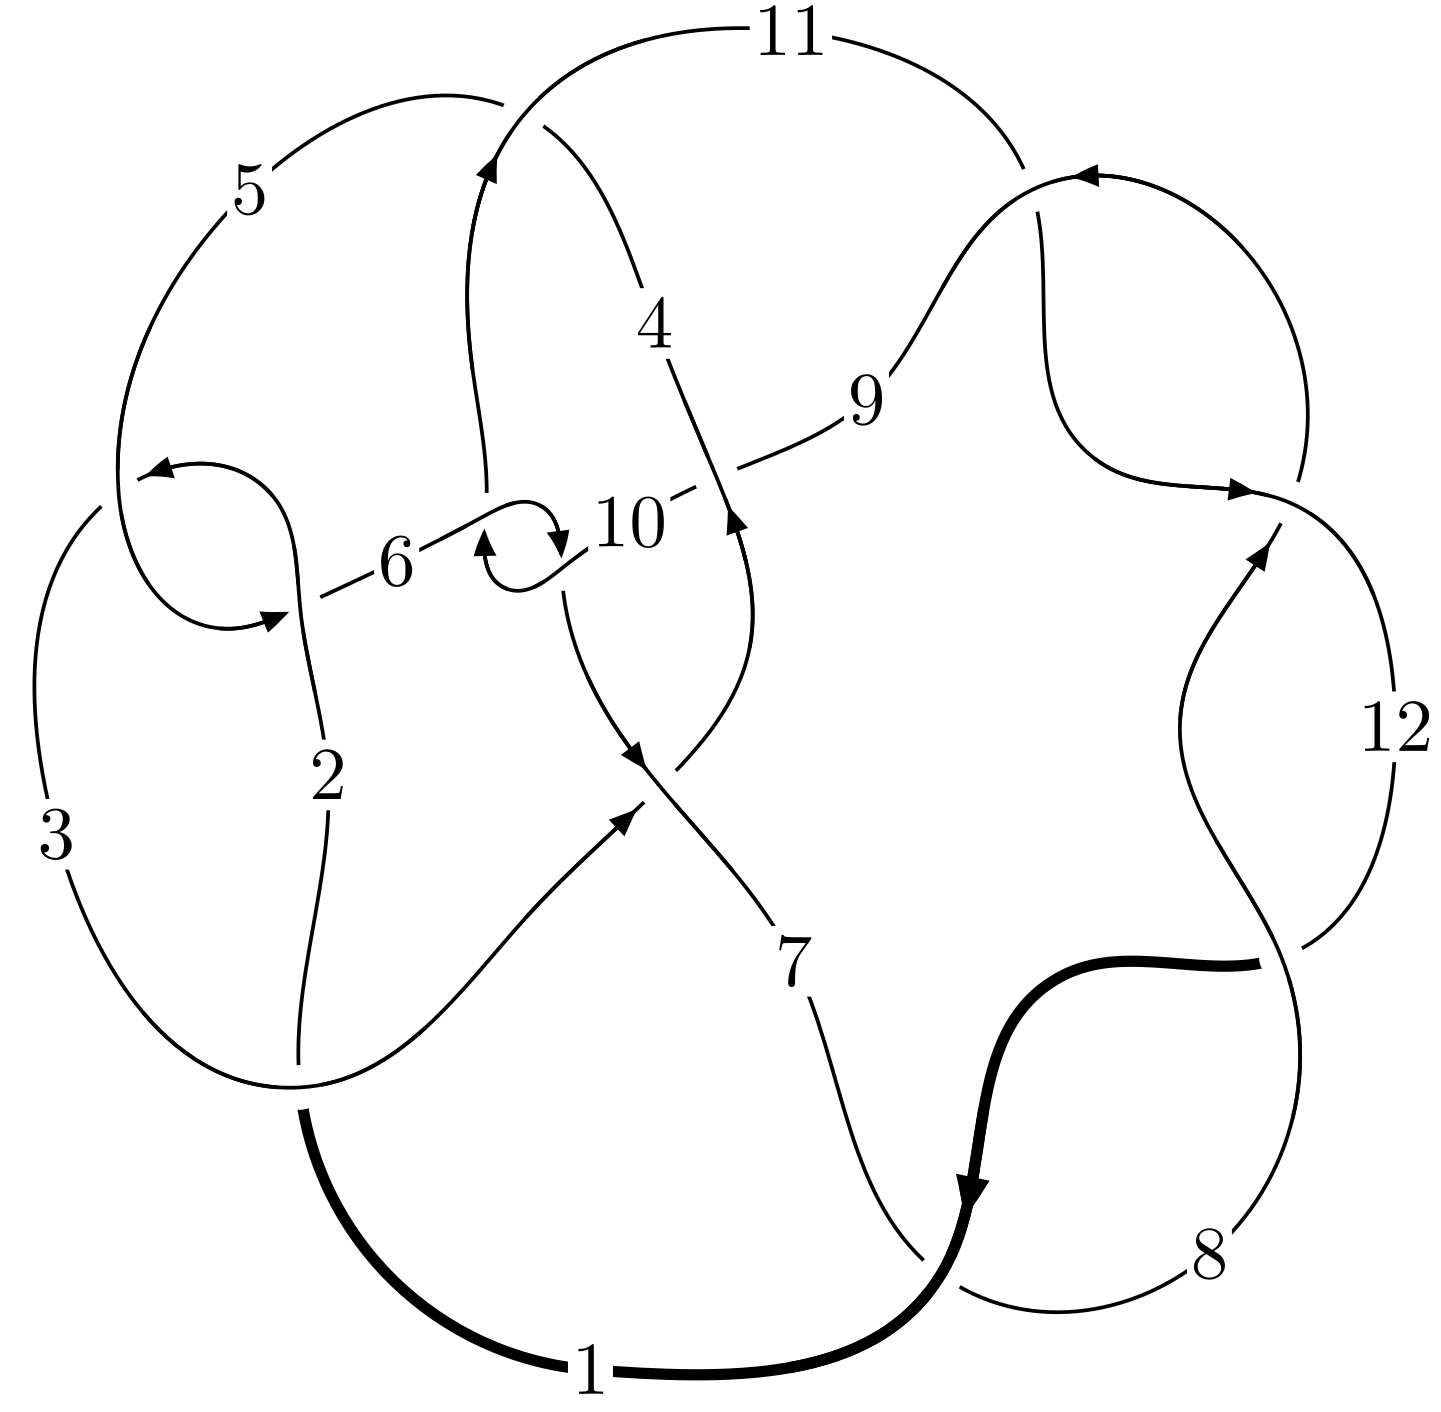
\includegraphics[width=112pt]{../../../GIT/diagram.site/Diagrams/png/877_12a_0076.png}\\
\ \ \ A knot diagram\footnotemark}&
\allowdisplaybreaks
\textbf{Linearized knot diagam} \\
\cline{2-2}
 &
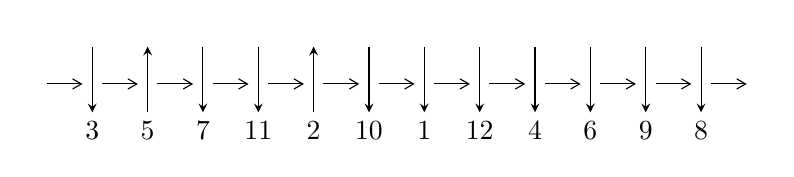
\begin{tikzpicture}[x=20pt, y=17pt]
	% nodes
	\node (C0) at (0, 0) {};
	\node (C1) at (1, 0) {};
	\node (C1U) at (1, +1) {};
	\node (C1D) at (1, -1) {3};

	\node (C2) at (2, 0) {};
	\node (C2U) at (2, +1) {};
	\node (C2D) at (2, -1) {5};

	\node (C3) at (3, 0) {};
	\node (C3U) at (3, +1) {};
	\node (C3D) at (3, -1) {7};

	\node (C4) at (4, 0) {};
	\node (C4U) at (4, +1) {};
	\node (C4D) at (4, -1) {11};

	\node (C5) at (5, 0) {};
	\node (C5U) at (5, +1) {};
	\node (C5D) at (5, -1) {2};

	\node (C6) at (6, 0) {};
	\node (C6U) at (6, +1) {};
	\node (C6D) at (6, -1) {10};

	\node (C7) at (7, 0) {};
	\node (C7U) at (7, +1) {};
	\node (C7D) at (7, -1) {1};

	\node (C8) at (8, 0) {};
	\node (C8U) at (8, +1) {};
	\node (C8D) at (8, -1) {12};

	\node (C9) at (9, 0) {};
	\node (C9U) at (9, +1) {};
	\node (C9D) at (9, -1) {4};

	\node (C10) at (10, 0) {};
	\node (C10U) at (10, +1) {};
	\node (C10D) at (10, -1) {6};

	\node (C11) at (11, 0) {};
	\node (C11U) at (11, +1) {};
	\node (C11D) at (11, -1) {9};

	\node (C12) at (12, 0) {};
	\node (C12U) at (12, +1) {};
	\node (C12D) at (12, -1) {8};
	\node (C13) at (13, 0) {};

	% arrows
	\draw[->,>={angle 60}]
	(C0) edge (C1) (C1) edge (C2) (C2) edge (C3) (C3) edge (C4) (C4) edge (C5) (C5) edge (C6) (C6) edge (C7) (C7) edge (C8) (C8) edge (C9) (C9) edge (C10) (C10) edge (C11) (C11) edge (C12) (C12) edge (C13) ;	\draw[->,>=stealth]
	(C1U) edge (C1D) (C2D) edge (C2U) (C3U) edge (C3D) (C4U) edge (C4D) (C5D) edge (C5U) (C6U) edge (C6D) (C7U) edge (C7D) (C8U) edge (C8D) (C9U) edge (C9D) (C10U) edge (C10D) (C11U) edge (C11D) (C12U) edge (C12D) ;
	\end{tikzpicture} \\
\hhline{~~} \\& 
\textbf{Solving Sequence} \\ \cline{2-2} 
 &
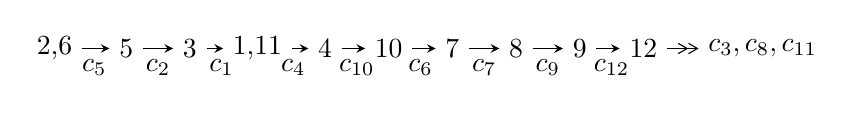
\begin{tikzpicture}[x=23pt, y=7pt]
	% node
	\node (A0) at (-1/8, 0) {2,6};
	\node (A1) at (1, 0) {5};
	\node (A2) at (2, 0) {3};
	\node (A3) at (49/16, 0) {1,11};
	\node (A4) at (33/8, 0) {4};
	\node (A5) at (41/8, 0) {10};
	\node (A6) at (49/8, 0) {7};
	\node (A7) at (57/8, 0) {8};
	\node (A8) at (65/8, 0) {9};
	\node (A9) at (73/8, 0) {12};
	\node (C1) at (1/2, -1) {$c_{5}$};
	\node (C2) at (3/2, -1) {$c_{2}$};
	\node (C3) at (5/2, -1) {$c_{1}$};
	\node (C4) at (29/8, -1) {$c_{4}$};
	\node (C5) at (37/8, -1) {$c_{10}$};
	\node (C6) at (45/8, -1) {$c_{6}$};
	\node (C7) at (53/8, -1) {$c_{7}$};
	\node (C8) at (61/8, -1) {$c_{9}$};
	\node (C9) at (69/8, -1) {$c_{12}$};
	\node (A10) at (11, 0) {$c_{3},c_{8},c_{11}$};

	% edge
	\draw[->,>=stealth]	
	(A0) edge (A1) (A1) edge (A2) (A2) edge (A3) (A3) edge (A4) (A4) edge (A5) (A5) edge (A6) (A6) edge (A7) (A7) edge (A8) (A8) edge (A9) ;
	\draw[->>,>={angle 60}]	
	(A9) edge (A10);
\end{tikzpicture} \\ 

\end{tabular} \\

\footnotetext{
The image of knot diagram is generated by the software ``\textbf{Draw programme}" developed by Andrew Bartholomew(\url{http://www.layer8.co.uk/maths/draw/index.htm\#Running-draw}), where we modified some parts for our purpose(\url{https://github.com/CATsTAILs/LinksPainter}).
}\phantom \\ \newline 
\centering \textbf{Ideals for irreducible components\footnotemark of $X_{\text{par}}$} 
 
\begin{align*}
I^u_{1}&=\langle 
7.93101\times10^{98} u^{76}+1.64483\times10^{99} u^{75}+\cdots+2.50573\times10^{99} b-1.01951\times10^{100},\\
\phantom{I^u_{1}}&\phantom{= \langle  }-2.37414\times10^{100} u^{76}-7.33884\times10^{100} u^{75}+\cdots+6.26432\times10^{100} a-4.38701\times10^{101},\\
\phantom{I^u_{1}}&\phantom{= \langle  }u^{77}+4 u^{76}+\cdots+101 u+25\rangle \\
I^u_{2}&=\langle 
-320 a^2 u-190 a^2-889 a u+1993 b+1652 a+701 u-518,\;5 a^3-5 a^2 u-4 a^2-4 a u- a+11 u-11,\\
\phantom{I^u_{2}}&\phantom{= \langle  }u^2- u+1\rangle \\
\\
\end{align*}
\raggedright * 2 irreducible components of $\dim_{\mathbb{C}}=0$, with total 83 representations.\\
\footnotetext{All coefficients of polynomials are rational numbers. But the coefficients are sometimes approximated in decimal forms when there is not enough margin.}
\newpage
\renewcommand{\arraystretch}{1}
\centering \section*{I. $I^u_{1}= \langle 7.93\times10^{98} u^{76}+1.64\times10^{99} u^{75}+\cdots+2.51\times10^{99} b-1.02\times10^{100},\;-2.37\times10^{100} u^{76}-7.34\times10^{100} u^{75}+\cdots+6.26\times10^{100} a-4.39\times10^{101},\;u^{77}+4 u^{76}+\cdots+101 u+25 \rangle$}
\flushleft \textbf{(i) Arc colorings}\\
\begin{tabular}{m{7pt} m{180pt} m{7pt} m{180pt} }
\flushright $a_{2}=$&$\begin{pmatrix}0\\u\end{pmatrix}$ \\
\flushright $a_{6}=$&$\begin{pmatrix}1\\0\end{pmatrix}$ \\
\flushright $a_{5}=$&$\begin{pmatrix}1\\u^2\end{pmatrix}$ \\
\flushright $a_{3}=$&$\begin{pmatrix}u\\u^3+u\end{pmatrix}$ \\
\flushright $a_{1}=$&$\begin{pmatrix}u^3\\u^5+u^3+u\end{pmatrix}$ \\
\flushright $a_{11}=$&$\begin{pmatrix}0.378995 u^{76}+1.17153 u^{75}+\cdots+38.9689 u+7.00317\\-0.316515 u^{76}-0.656426 u^{75}+\cdots+3.88281 u+4.06872\end{pmatrix}$ \\
\flushright $a_{4}=$&$\begin{pmatrix}0.382922 u^{76}+1.34261 u^{75}+\cdots+5.59826 u+1.24813\\0.316632 u^{76}+1.34041 u^{75}+\cdots+40.8488 u+10.7971\end{pmatrix}$ \\
\flushright $a_{10}=$&$\begin{pmatrix}0.0624796 u^{76}+0.515104 u^{75}+\cdots+42.8517 u+11.0719\\-0.316515 u^{76}-0.656426 u^{75}+\cdots+3.88281 u+4.06872\end{pmatrix}$ \\
\flushright $a_{7}=$&$\begin{pmatrix}0.169032 u^{76}-0.182910 u^{75}+\cdots-24.2572 u-6.80526\\0.289827 u^{76}+0.617219 u^{75}+\cdots-5.81712 u-2.87335\end{pmatrix}$ \\
\flushright $a_{8}=$&$\begin{pmatrix}0.172862 u^{76}-0.154859 u^{75}+\cdots-23.2157 u-6.96987\\0.326324 u^{76}+0.494996 u^{75}+\cdots-15.9347 u-6.46441\end{pmatrix}$ \\
\flushright $a_{9}=$&$\begin{pmatrix}-0.155679 u^{76}-0.308708 u^{75}+\cdots+14.0992 u+4.25438\\-0.0753730 u^{76}-0.185600 u^{75}+\cdots+1.65389 u+2.31494\end{pmatrix}$ \\
\flushright $a_{12}=$&$\begin{pmatrix}0.241155 u^{76}+0.606307 u^{75}+\cdots-6.10719 u-4.25876\\0.00962114 u^{76}+0.358023 u^{75}+\cdots+14.6700 u+3.86949\end{pmatrix}$\\&\end{tabular}
\flushleft \textbf{(ii) Obstruction class $= -1$}\\~\\
\flushleft \textbf{(iii) Cusp Shapes $= -1.55122 u^{76}-3.85524 u^{75}+\cdots-10.1221 u+0.155354$}\\~\\
\newpage\renewcommand{\arraystretch}{1}
\flushleft \textbf{(iv) u-Polynomials at the component}\newline \\
\begin{tabular}{m{50pt}|m{274pt}}
Crossings & \hspace{64pt}u-Polynomials at each crossing \\
\hline $$\begin{aligned}c_{1}\end{aligned}$$&$\begin{aligned}
&u^{77}+26 u^{76}+\cdots+4801 u-625
\end{aligned}$\\
\hline $$\begin{aligned}c_{2},c_{5}\end{aligned}$$&$\begin{aligned}
&u^{77}+4 u^{76}+\cdots+101 u+25
\end{aligned}$\\
\hline $$\begin{aligned}c_{3}\end{aligned}$$&$\begin{aligned}
&25(25 u^{77}-140 u^{76}+\cdots-1.87152\times10^{7} u+4199891)
\end{aligned}$\\
\hline $$\begin{aligned}c_{4}\end{aligned}$$&$\begin{aligned}
&25(25 u^{77}-45 u^{76}+\cdots+49984 u+52544)
\end{aligned}$\\
\hline $$\begin{aligned}c_{6},c_{10}\end{aligned}$$&$\begin{aligned}
&u^{77}+3 u^{76}+\cdots-8 u^2+1
\end{aligned}$\\
\hline $$\begin{aligned}c_{7},c_{8},c_{11}\\c_{12}\end{aligned}$$&$\begin{aligned}
&u^{77}-3 u^{76}+\cdots-6 u+1
\end{aligned}$\\
\hline $$\begin{aligned}c_{9}\end{aligned}$$&$\begin{aligned}
&u^{77}+u^{76}+\cdots+15200 u+8000
\end{aligned}$\\
\hline
\end{tabular}\\~\\
\newpage\renewcommand{\arraystretch}{1}
\flushleft \textbf{(v) Riley Polynomials at the component}\newline \\
\begin{tabular}{m{50pt}|m{274pt}}
Crossings & \hspace{64pt}Riley Polynomials at each crossing \\
\hline $$\begin{aligned}c_{1}\end{aligned}$$&$\begin{aligned}
&y^{77}+54 y^{76}+\cdots+264859601 y-390625
\end{aligned}$\\
\hline $$\begin{aligned}c_{2},c_{5}\end{aligned}$$&$\begin{aligned}
&y^{77}+26 y^{76}+\cdots+4801 y-625
\end{aligned}$\\
\hline $$\begin{aligned}c_{3}\end{aligned}$$&$\begin{aligned}
&625\\
&\cdot(625 y^{77}+32100 y^{76}+\cdots-165791891422930 y-17639084411881)
\end{aligned}$\\
\hline $$\begin{aligned}c_{4}\end{aligned}$$&$\begin{aligned}
&625(625 y^{77}+30025 y^{76}+\cdots-4.56084\times10^{10} y-2.76087\times10^{9})
\end{aligned}$\\
\hline $$\begin{aligned}c_{6},c_{10}\end{aligned}$$&$\begin{aligned}
&y^{77}+49 y^{76}+\cdots+16 y-1
\end{aligned}$\\
\hline $$\begin{aligned}c_{7},c_{8},c_{11}\\c_{12}\end{aligned}$$&$\begin{aligned}
&y^{77}+93 y^{76}+\cdots+16 y-1
\end{aligned}$\\
\hline $$\begin{aligned}c_{9}\end{aligned}$$&$\begin{aligned}
&y^{77}+35 y^{76}+\cdots-964480000 y-64000000
\end{aligned}$\\
\hline
\end{tabular}\\~\\
\newpage\flushleft \textbf{(vi) Complex Volumes and Cusp Shapes}
$$\begin{array}{c|c|c}  
\text{Solutions to }I^u_{1}& \I (\text{vol} + \sqrt{-1}CS) & \text{Cusp shape}\\
 \hline 
\begin{aligned}
u &= \phantom{-}0.023387 + 0.993675 I \\
a &= -1.48275 + 0.20664 I \\
b &= \phantom{-}0.625759 + 0.325187 I\end{aligned}
 & -1.74432 + 2.06267 I & \phantom{-0.000000 } 0 \\ \hline\begin{aligned}
u &= \phantom{-}0.023387 - 0.993675 I \\
a &= -1.48275 - 0.20664 I \\
b &= \phantom{-}0.625759 - 0.325187 I\end{aligned}
 & -1.74432 - 2.06267 I & \phantom{-0.000000 } 0 \\ \hline\begin{aligned}
u &= -0.689051 + 0.710247 I \\
a &= -0.672174 + 0.847004 I \\
b &= \phantom{-}1.093650 - 0.218602 I\end{aligned}
 & \phantom{-}3.26103 + 2.04999 I & \phantom{-0.000000 } 0 \\ \hline\begin{aligned}
u &= -0.689051 - 0.710247 I \\
a &= -0.672174 - 0.847004 I \\
b &= \phantom{-}1.093650 + 0.218602 I\end{aligned}
 & \phantom{-}3.26103 - 2.04999 I & \phantom{-0.000000 } 0 \\ \hline\begin{aligned}
u &= \phantom{-}0.437005 + 0.886797 I \\
a &= -0.617746 - 0.137414 I \\
b &= \phantom{-}0.200968 + 0.136308 I\end{aligned}
 & -0.31514 + 1.81008 I & \phantom{-0.000000 } 0 \\ \hline\begin{aligned}
u &= \phantom{-}0.437005 - 0.886797 I \\
a &= -0.617746 + 0.137414 I \\
b &= \phantom{-}0.200968 - 0.136308 I\end{aligned}
 & -0.31514 - 1.81008 I & \phantom{-0.000000 } 0 \\ \hline\begin{aligned}
u &= -0.802987 + 0.670328 I \\
a &= -0.132409 + 0.135406 I \\
b &= -0.43177 + 1.42400 I\end{aligned}
 & \phantom{-}5.18414 + 3.21854 I & \phantom{-0.000000 } 0 \\ \hline\begin{aligned}
u &= -0.802987 - 0.670328 I \\
a &= -0.132409 - 0.135406 I \\
b &= -0.43177 - 1.42400 I\end{aligned}
 & \phantom{-}5.18414 - 3.21854 I & \phantom{-0.000000 } 0 \\ \hline\begin{aligned}
u &= \phantom{-}0.580300 + 0.745312 I \\
a &= \phantom{-}0.01473 + 1.95275 I \\
b &= -0.032548 + 1.130350 I\end{aligned}
 & \phantom{-}2.99487 + 1.53571 I & -8.00000 + 0. I\phantom{ +0.000000I} \\ \hline\begin{aligned}
u &= \phantom{-}0.580300 - 0.745312 I \\
a &= \phantom{-}0.01473 - 1.95275 I \\
b &= -0.032548 - 1.130350 I\end{aligned}
 & \phantom{-}2.99487 - 1.53571 I & -8.00000 + 0. I\phantom{ +0.000000I}\\
 \hline 
 \end{array}$$\newpage$$\begin{array}{c|c|c}  
\text{Solutions to }I^u_{1}& \I (\text{vol} + \sqrt{-1}CS) & \text{Cusp shape}\\
 \hline 
\begin{aligned}
u &= -0.850071 + 0.645897 I \\
a &= \phantom{-}0.687278 - 0.617056 I \\
b &= -1.031170 + 0.139364 I\end{aligned}
 & \phantom{-}12.61110 + 4.44495 I & \phantom{-0.000000 } 0 \\ \hline\begin{aligned}
u &= -0.850071 - 0.645897 I \\
a &= \phantom{-}0.687278 + 0.617056 I \\
b &= -1.031170 - 0.139364 I\end{aligned}
 & \phantom{-}12.61110 - 4.44495 I & \phantom{-0.000000 } 0 \\ \hline\begin{aligned}
u &= \phantom{-}0.107724 + 1.076330 I \\
a &= \phantom{-}0.83445 - 1.21670 I \\
b &= -0.391468 + 0.997418 I\end{aligned}
 & -1.08919 + 2.96820 I & \phantom{-0.000000 } 0 \\ \hline\begin{aligned}
u &= \phantom{-}0.107724 - 1.076330 I \\
a &= \phantom{-}0.83445 + 1.21670 I \\
b &= -0.391468 - 0.997418 I\end{aligned}
 & -1.08919 - 2.96820 I & \phantom{-0.000000 } 0 \\ \hline\begin{aligned}
u &= -0.645982 + 0.868158 I \\
a &= \phantom{-}0.960269 - 0.964614 I \\
b &= -1.243670 + 0.117565 I\end{aligned}
 & -0.13971 - 2.51501 I & \phantom{-0.000000 } 0 \\ \hline\begin{aligned}
u &= -0.645982 - 0.868158 I \\
a &= \phantom{-}0.960269 + 0.964614 I \\
b &= -1.243670 - 0.117565 I\end{aligned}
 & -0.13971 + 2.51501 I & \phantom{-0.000000 } 0 \\ \hline\begin{aligned}
u &= -0.756836 + 0.799522 I \\
a &= \phantom{-}0.201274 + 0.141714 I \\
b &= \phantom{-}0.47634 - 1.45900 I\end{aligned}
 & \phantom{-}7.35750 - 1.25503 I & \phantom{-0.000000 } 0 \\ \hline\begin{aligned}
u &= -0.756836 - 0.799522 I \\
a &= \phantom{-}0.201274 - 0.141714 I \\
b &= \phantom{-}0.47634 + 1.45900 I\end{aligned}
 & \phantom{-}7.35750 + 1.25503 I & \phantom{-0.000000 } 0 \\ \hline\begin{aligned}
u &= -0.925906 + 0.617713 I \\
a &= -0.094308 - 0.190665 I \\
b &= \phantom{-}0.44275 - 1.38890 I\end{aligned}
 & \phantom{-}8.30126 + 7.27195 I & \phantom{-0.000000 } 0 \\ \hline\begin{aligned}
u &= -0.925906 - 0.617713 I \\
a &= -0.094308 + 0.190665 I \\
b &= \phantom{-}0.44275 + 1.38890 I\end{aligned}
 & \phantom{-}8.30126 - 7.27195 I & \phantom{-0.000000 } 0\\
 \hline 
 \end{array}$$\newpage$$\begin{array}{c|c|c}  
\text{Solutions to }I^u_{1}& \I (\text{vol} + \sqrt{-1}CS) & \text{Cusp shape}\\
 \hline 
\begin{aligned}
u &= -0.171129 + 0.864991 I \\
a &= \phantom{-}1.77593 - 0.38376 I \\
b &= -0.748125 - 0.526560 I\end{aligned}
 & -2.60922 - 1.38173 I & -13.51813 + 2.09755 I \\ \hline\begin{aligned}
u &= -0.171129 - 0.864991 I \\
a &= \phantom{-}1.77593 + 0.38376 I \\
b &= -0.748125 + 0.526560 I\end{aligned}
 & -2.60922 + 1.38173 I & -13.51813 - 2.09755 I \\ \hline\begin{aligned}
u &= \phantom{-}0.564948 + 0.667315 I \\
a &= -1.52137 - 2.48650 I \\
b &= \phantom{-}0.111660 + 0.733444 I\end{aligned}
 & \phantom{-}10.81200 + 1.40949 I & -6.43106 - 2.48150 I \\ \hline\begin{aligned}
u &= \phantom{-}0.564948 - 0.667315 I \\
a &= -1.52137 + 2.48650 I \\
b &= \phantom{-}0.111660 - 0.733444 I\end{aligned}
 & \phantom{-}10.81200 - 1.40949 I & -6.43106 + 2.48150 I \\ \hline\begin{aligned}
u &= \phantom{-}0.582271 + 0.971594 I \\
a &= \phantom{-}0.641231 - 0.469572 I \\
b &= -0.301785 + 0.108520 I\end{aligned}
 & \phantom{-}1.27808 + 3.12805 I & \phantom{-0.000000 } 0 \\ \hline\begin{aligned}
u &= \phantom{-}0.582271 - 0.971594 I \\
a &= \phantom{-}0.641231 + 0.469572 I \\
b &= -0.301785 - 0.108520 I\end{aligned}
 & \phantom{-}1.27808 - 3.12805 I & \phantom{-0.000000 } 0 \\ \hline\begin{aligned}
u &= -0.378177 + 0.760297 I \\
a &= -1.97319 + 0.66535 I \\
b &= \phantom{-}0.893170 + 0.851679 I\end{aligned}
 & \phantom{-}2.80627 - 4.33786 I & -7.45487 - 3.06969 I \\ \hline\begin{aligned}
u &= -0.378177 - 0.760297 I \\
a &= -1.97319 - 0.66535 I \\
b &= \phantom{-}0.893170 - 0.851679 I\end{aligned}
 & \phantom{-}2.80627 + 4.33786 I & -7.45487 + 3.06969 I \\ \hline\begin{aligned}
u &= -0.790859 + 0.836843 I \\
a &= \phantom{-}1.77041 - 0.38931 I \\
b &= -0.62234 - 1.33323 I\end{aligned}
 & \phantom{-}16.1641 - 1.5411 I & \phantom{-0.000000 } 0 \\ \hline\begin{aligned}
u &= -0.790859 - 0.836843 I \\
a &= \phantom{-}1.77041 + 0.38931 I \\
b &= -0.62234 + 1.33323 I\end{aligned}
 & \phantom{-}16.1641 + 1.5411 I & \phantom{-0.000000 } 0\\
 \hline 
 \end{array}$$\newpage$$\begin{array}{c|c|c}  
\text{Solutions to }I^u_{1}& \I (\text{vol} + \sqrt{-1}CS) & \text{Cusp shape}\\
 \hline 
\begin{aligned}
u &= \phantom{-}0.639240 + 0.976315 I \\
a &= -1.65830 - 0.49768 I \\
b &= \phantom{-}0.125080 - 1.109880 I\end{aligned}
 & \phantom{-}2.18376 + 3.33368 I & \phantom{-0.000000 } 0 \\ \hline\begin{aligned}
u &= \phantom{-}0.639240 - 0.976315 I \\
a &= -1.65830 + 0.49768 I \\
b &= \phantom{-}0.125080 + 1.109880 I\end{aligned}
 & \phantom{-}2.18376 - 3.33368 I & \phantom{-0.000000 } 0 \\ \hline\begin{aligned}
u &= \phantom{-}0.283439 + 0.778804 I \\
a &= \phantom{-}2.33704 - 1.18812 I \\
b &= -0.062296 - 1.174070 I\end{aligned}
 & \phantom{-}9.98727 + 1.50639 I & -0.66145 - 3.42901 I \\ \hline\begin{aligned}
u &= \phantom{-}0.283439 - 0.778804 I \\
a &= \phantom{-}2.33704 + 1.18812 I \\
b &= -0.062296 + 1.174070 I\end{aligned}
 & \phantom{-}9.98727 - 1.50639 I & -0.66145 + 3.42901 I \\ \hline\begin{aligned}
u &= \phantom{-}0.117920 + 1.168920 I \\
a &= \phantom{-}1.291680 - 0.300778 I \\
b &= -0.628830 - 0.167135 I\end{aligned}
 & \phantom{-}5.79410 + 3.63952 I & \phantom{-0.000000 } 0 \\ \hline\begin{aligned}
u &= \phantom{-}0.117920 - 1.168920 I \\
a &= \phantom{-}1.291680 + 0.300778 I \\
b &= -0.628830 + 0.167135 I\end{aligned}
 & \phantom{-}5.79410 - 3.63952 I & \phantom{-0.000000 } 0 \\ \hline\begin{aligned}
u &= -0.723744 + 0.928946 I \\
a &= -1.85578 + 0.31129 I \\
b &= \phantom{-}0.61575 + 1.38912 I\end{aligned}
 & \phantom{-}6.95838 - 4.36192 I & \phantom{-0.000000 } 0 \\ \hline\begin{aligned}
u &= -0.723744 - 0.928946 I \\
a &= -1.85578 - 0.31129 I \\
b &= \phantom{-}0.61575 - 1.38912 I\end{aligned}
 & \phantom{-}6.95838 + 4.36192 I & \phantom{-0.000000 } 0 \\ \hline\begin{aligned}
u &= \phantom{-}1.082260 + 0.468850 I \\
a &= -0.123493 - 0.256538 I \\
b &= \phantom{-}0.044273 - 1.217200 I\end{aligned}
 & \phantom{-}6.73924 + 1.85246 I & \phantom{-0.000000 } 0 \\ \hline\begin{aligned}
u &= \phantom{-}1.082260 - 0.468850 I \\
a &= -0.123493 + 0.256538 I \\
b &= \phantom{-}0.044273 + 1.217200 I\end{aligned}
 & \phantom{-}6.73924 - 1.85246 I & \phantom{-0.000000 } 0\\
 \hline 
 \end{array}$$\newpage$$\begin{array}{c|c|c}  
\text{Solutions to }I^u_{1}& \I (\text{vol} + \sqrt{-1}CS) & \text{Cusp shape}\\
 \hline 
\begin{aligned}
u &= -0.676567 + 0.972926 I \\
a &= -1.098660 + 0.822983 I \\
b &= \phantom{-}1.181550 - 0.009799 I\end{aligned}
 & \phantom{-}2.47138 - 7.34623 I & \phantom{-0.000000 } 0 \\ \hline\begin{aligned}
u &= -0.676567 - 0.972926 I \\
a &= -1.098660 - 0.822983 I \\
b &= \phantom{-}1.181550 + 0.009799 I\end{aligned}
 & \phantom{-}2.47138 + 7.34623 I & \phantom{-0.000000 } 0 \\ \hline\begin{aligned}
u &= -1.025320 + 0.614382 I \\
a &= \phantom{-}0.228092 + 0.157777 I \\
b &= -0.45532 + 1.37631 I\end{aligned}
 & \phantom{-}17.3658 + 9.6655 I & \phantom{-0.000000 } 0 \\ \hline\begin{aligned}
u &= -1.025320 - 0.614382 I \\
a &= \phantom{-}0.228092 - 0.157777 I \\
b &= -0.45532 - 1.37631 I\end{aligned}
 & \phantom{-}17.3658 - 9.6655 I & \phantom{-0.000000 } 0 \\ \hline\begin{aligned}
u &= -0.769678 + 0.915176 I \\
a &= -0.069711 - 0.333527 I \\
b &= -0.52438 + 1.43530 I\end{aligned}
 & \phantom{-}15.9240 - 4.3215 I & \phantom{-0.000000 } 0 \\ \hline\begin{aligned}
u &= -0.769678 - 0.915176 I \\
a &= -0.069711 + 0.333527 I \\
b &= -0.52438 - 1.43530 I\end{aligned}
 & \phantom{-}15.9240 + 4.3215 I & \phantom{-0.000000 } 0 \\ \hline\begin{aligned}
u &= \phantom{-}0.457284 + 0.657961 I \\
a &= \phantom{-}0.61765 + 1.70350 I \\
b &= -0.013064 - 0.547144 I\end{aligned}
 & \phantom{-}2.28018 + 1.37290 I & -3.34311 - 4.48860 I \\ \hline\begin{aligned}
u &= \phantom{-}0.457284 - 0.657961 I \\
a &= \phantom{-}0.61765 - 1.70350 I \\
b &= -0.013064 + 0.547144 I\end{aligned}
 & \phantom{-}2.28018 - 1.37290 I & -3.34311 + 4.48860 I \\ \hline\begin{aligned}
u &= -0.271251 + 0.735692 I \\
a &= -0.256281 + 1.284760 I \\
b &= \phantom{-}0.764229 - 0.712502 I\end{aligned}
 & \phantom{-}2.74924 + 1.47081 I & -7.37057 - 5.74659 I \\ \hline\begin{aligned}
u &= -0.271251 - 0.735692 I \\
a &= -0.256281 - 1.284760 I \\
b &= \phantom{-}0.764229 + 0.712502 I\end{aligned}
 & \phantom{-}2.74924 - 1.47081 I & -7.37057 + 5.74659 I\\
 \hline 
 \end{array}$$\newpage$$\begin{array}{c|c|c}  
\text{Solutions to }I^u_{1}& \I (\text{vol} + \sqrt{-1}CS) & \text{Cusp shape}\\
 \hline 
\begin{aligned}
u &= \phantom{-}0.672668 + 1.026560 I \\
a &= -0.772233 + 0.609784 I \\
b &= \phantom{-}0.372498 - 0.168400 I\end{aligned}
 & \phantom{-}9.55875 + 3.71126 I & \phantom{-0.000000 } 0 \\ \hline\begin{aligned}
u &= \phantom{-}0.672668 - 1.026560 I \\
a &= -0.772233 - 0.609784 I \\
b &= \phantom{-}0.372498 + 0.168400 I\end{aligned}
 & \phantom{-}9.55875 - 3.71126 I & \phantom{-0.000000 } 0 \\ \hline\begin{aligned}
u &= -0.712145 + 1.018770 I \\
a &= \phantom{-}1.86345 - 0.22946 I \\
b &= -0.57025 - 1.40468 I\end{aligned}
 & \phantom{-}4.13125 - 8.92679 I & \phantom{-0.000000 } 0 \\ \hline\begin{aligned}
u &= -0.712145 - 1.018770 I \\
a &= \phantom{-}1.86345 + 0.22946 I \\
b &= -0.57025 + 1.40468 I\end{aligned}
 & \phantom{-}4.13125 + 8.92679 I & \phantom{-0.000000 } 0 \\ \hline\begin{aligned}
u &= \phantom{-}0.640073 + 0.401249 I \\
a &= \phantom{-}0.61346 - 1.74507 I \\
b &= -0.242727 + 0.508756 I\end{aligned}
 & \phantom{-}10.92250 + 1.41966 I & -3.27349 - 3.63147 I \\ \hline\begin{aligned}
u &= \phantom{-}0.640073 - 0.401249 I \\
a &= \phantom{-}0.61346 + 1.74507 I \\
b &= -0.242727 - 0.508756 I\end{aligned}
 & \phantom{-}10.92250 - 1.41966 I & -3.27349 + 3.63147 I \\ \hline\begin{aligned}
u &= -0.725026 + 1.045960 I \\
a &= \phantom{-}1.119890 - 0.723073 I \\
b &= -1.123130 - 0.004421 I\end{aligned}
 & \phantom{-}11.3969 - 10.3217 I & \phantom{-0.000000 } 0 \\ \hline\begin{aligned}
u &= -0.725026 - 1.045960 I \\
a &= \phantom{-}1.119890 + 0.723073 I \\
b &= -1.123130 + 0.004421 I\end{aligned}
 & \phantom{-}11.3969 + 10.3217 I & \phantom{-0.000000 } 0 \\ \hline\begin{aligned}
u &= \phantom{-}0.201201 + 1.271660 I \\
a &= -0.929381 + 0.895259 I \\
b &= \phantom{-}0.346853 - 1.094610 I\end{aligned}
 & \phantom{-}0.58610 + 5.84122 I & \phantom{-0.000000 } 0 \\ \hline\begin{aligned}
u &= \phantom{-}0.201201 - 1.271660 I \\
a &= -0.929381 - 0.895259 I \\
b &= \phantom{-}0.346853 + 1.094610 I\end{aligned}
 & \phantom{-}0.58610 - 5.84122 I & \phantom{-0.000000 } 0\\
 \hline 
 \end{array}$$\newpage$$\begin{array}{c|c|c}  
\text{Solutions to }I^u_{1}& \I (\text{vol} + \sqrt{-1}CS) & \text{Cusp shape}\\
 \hline 
\begin{aligned}
u &= -0.740013 + 1.082960 I \\
a &= -1.83895 + 0.18377 I \\
b &= \phantom{-}0.54663 + 1.38812 I\end{aligned}
 & \phantom{-}6.8662 - 13.3948 I & \phantom{-0.000000 } 0 \\ \hline\begin{aligned}
u &= -0.740013 - 1.082960 I \\
a &= -1.83895 - 0.18377 I \\
b &= \phantom{-}0.54663 - 1.38812 I\end{aligned}
 & \phantom{-}6.8662 + 13.3948 I & \phantom{-0.000000 } 0 \\ \hline\begin{aligned}
u &= -0.771024 + 1.128770 I \\
a &= \phantom{-}1.81769 - 0.15434 I \\
b &= -0.53700 - 1.37405 I\end{aligned}
 & \phantom{-}15.7376 - 16.1737 I & \phantom{-0.000000 } 0 \\ \hline\begin{aligned}
u &= -0.771024 - 1.128770 I \\
a &= \phantom{-}1.81769 + 0.15434 I \\
b &= -0.53700 + 1.37405 I\end{aligned}
 & \phantom{-}15.7376 + 16.1737 I & \phantom{-0.000000 } 0 \\ \hline\begin{aligned}
u &= \phantom{-}0.320237 + 0.541394 I \\
a &= -0.18136 + 2.01696 I \\
b &= \phantom{-}0.231553 - 0.595039 I\end{aligned}
 & \phantom{-}2.26536 + 1.35585 I & -3.06700 - 4.58945 I \\ \hline\begin{aligned}
u &= \phantom{-}0.320237 - 0.541394 I \\
a &= -0.18136 - 2.01696 I \\
b &= \phantom{-}0.231553 + 0.595039 I\end{aligned}
 & \phantom{-}2.26536 - 1.35585 I & -3.06700 + 4.58945 I \\ \hline\begin{aligned}
u &= \phantom{-}1.296830 + 0.495291 I \\
a &= \phantom{-}0.176059 + 0.133103 I \\
b &= -0.049062 + 1.240290 I\end{aligned}
 & \phantom{-}15.6374 + 2.0891 I & \phantom{-0.000000 } 0 \\ \hline\begin{aligned}
u &= \phantom{-}1.296830 - 0.495291 I \\
a &= \phantom{-}0.176059 - 0.133103 I \\
b &= -0.049062 - 1.240290 I\end{aligned}
 & \phantom{-}15.6374 - 2.0891 I & \phantom{-0.000000 } 0 \\ \hline\begin{aligned}
u &= \phantom{-}0.825265 + 1.129010 I \\
a &= \phantom{-}0.971647 + 0.072412 I \\
b &= -0.154594 + 1.175390 I\end{aligned}
 & \phantom{-}4.80654 + 4.92929 I & \phantom{-0.000000 } 0 \\ \hline\begin{aligned}
u &= \phantom{-}0.825265 - 1.129010 I \\
a &= \phantom{-}0.971647 - 0.072412 I \\
b &= -0.154594 - 1.175390 I\end{aligned}
 & \phantom{-}4.80654 - 4.92929 I & \phantom{-0.000000 } 0\\
 \hline 
 \end{array}$$\newpage$$\begin{array}{c|c|c}  
\text{Solutions to }I^u_{1}& \I (\text{vol} + \sqrt{-1}CS) & \text{Cusp shape}\\
 \hline 
\begin{aligned}
u &= \phantom{-}0.512499 + 0.280972 I \\
a &= -0.726334 + 0.007761 I \\
b &= -0.013821 + 1.181210 I\end{aligned}
 & \phantom{-}3.20881 + 1.14210 I & -4.80285 - 5.42907 I \\ \hline\begin{aligned}
u &= \phantom{-}0.512499 - 0.280972 I \\
a &= -0.726334 - 0.007761 I \\
b &= -0.013821 - 1.181210 I\end{aligned}
 & \phantom{-}3.20881 - 1.14210 I & -4.80285 + 5.42907 I \\ \hline\begin{aligned}
u &= \phantom{-}0.23954 + 1.42224 I \\
a &= \phantom{-}0.869717 - 0.736081 I \\
b &= -0.336774 + 1.148260 I\end{aligned}
 & \phantom{-}8.71669 + 7.31926 I & \phantom{-0.000000 } 0 \\ \hline\begin{aligned}
u &= \phantom{-}0.23954 - 1.42224 I \\
a &= \phantom{-}0.869717 + 0.736081 I \\
b &= -0.336774 - 1.148260 I\end{aligned}
 & \phantom{-}8.71669 - 7.31926 I & \phantom{-0.000000 } 0 \\ \hline\begin{aligned}
u &= \phantom{-}0.93837 + 1.22898 I \\
a &= -0.807522 + 0.046238 I \\
b &= \phantom{-}0.163263 - 1.205750 I\end{aligned}
 & \phantom{-}13.4511 + 5.6875 I & \phantom{-0.000000 } 0 \\ \hline\begin{aligned}
u &= \phantom{-}0.93837 - 1.22898 I \\
a &= -0.807522 - 0.046238 I \\
b &= \phantom{-}0.163263 + 1.205750 I\end{aligned}
 & \phantom{-}13.4511 - 5.6875 I & \phantom{-0.000000 } 0 \\ \hline\begin{aligned}
u &= -0.193384\phantom{ +0.000000I} \\
a &= -1.47995\phantom{ +0.000000I} \\
b &= -0.443692\phantom{ +0.000000I}\end{aligned}
 & -0.677358\phantom{ +0.000000I} & -14.5420\phantom{ +0.000000I}\\
 \hline 
 \end{array}$$\newpage\newpage\renewcommand{\arraystretch}{1}
\centering \section*{II. $I^u_{2}= \langle -320 a^2 u-889 a u+\cdots+1652 a-518,\;5 a^3-5 a^2 u-4 a^2-4 a u- a+11 u-11,\;u^2- u+1 \rangle$}
\flushleft \textbf{(i) Arc colorings}\\
\begin{tabular}{m{7pt} m{180pt} m{7pt} m{180pt} }
\flushright $a_{2}=$&$\begin{pmatrix}0\\u\end{pmatrix}$ \\
\flushright $a_{6}=$&$\begin{pmatrix}1\\0\end{pmatrix}$ \\
\flushright $a_{5}=$&$\begin{pmatrix}1\\u-1\end{pmatrix}$ \\
\flushright $a_{3}=$&$\begin{pmatrix}u\\u-1\end{pmatrix}$ \\
\flushright $a_{1}=$&$\begin{pmatrix}-1\\0\end{pmatrix}$ \\
\flushright $a_{11}=$&$\begin{pmatrix}a\\0.160562 a^{2} u+0.446061 a u+\cdots-0.828901 a+0.259910\end{pmatrix}$ \\
\flushright $a_{4}=$&$\begin{pmatrix}0.169594 a^{2} u+0.114902 a u+\cdots-0.150527 a+0.437030\\-0.0326141 a^{2} u-0.137481 a u+\cdots+0.105871 a-0.584044\end{pmatrix}$ \\
\flushright $a_{10}=$&$\begin{pmatrix}0.160562 a^{2} u+0.446061 a u+\cdots+0.171099 a+0.259910\\0.160562 a^{2} u+0.446061 a u+\cdots-0.828901 a+0.259910\end{pmatrix}$ \\
\flushright $a_{7}=$&$\begin{pmatrix}-0.0501756 a^{2} u+0.173106 a u+\cdots+0.00903161 a+0.793778\\-0.880582 a^{2} u+0.288008 a u+\cdots-0.141495 a-0.769192\end{pmatrix}$ \\
\flushright $a_{8}=$&$\begin{pmatrix}0.830406 a^{2} u-0.114902 a u+\cdots+0.150527 a+1.56297\\-0.880582 a^{2} u+0.288008 a u+\cdots-0.141495 a-0.769192\end{pmatrix}$ \\
\flushright $a_{9}=$&$\begin{pmatrix}0.160562 a^{2} u+0.446061 a u+\cdots+0.171099 a+0.259910\\0.160562 a^{2} u+0.446061 a u+\cdots-0.828901 a+0.259910\end{pmatrix}$ \\
\flushright $a_{12}=$&$\begin{pmatrix}0.158053 a^{2} u+0.204717 a u+\cdots+0.871550 a-0.400401\\-0.720020 a^{2} u+0.734069 a u+\cdots-0.970396 a-1.50928\end{pmatrix}$\\&\end{tabular}
\flushleft \textbf{(ii) Obstruction class $= 1$}\\~\\
\flushleft \textbf{(iii) Cusp Shapes $= \frac{402}{1993} a^2 u-\frac{135}{1993} a^2-\frac{8761}{1993} a u+\frac{8936}{1993} a-\frac{10883}{1993} u-\frac{9389}{1993}$}\\~\\
\newpage\renewcommand{\arraystretch}{1}
\flushleft \textbf{(iv) u-Polynomials at the component}\newline \\
\begin{tabular}{m{50pt}|m{274pt}}
Crossings & \hspace{64pt}u-Polynomials at each crossing \\
\hline $$\begin{aligned}c_{1},c_{5}\end{aligned}$$&$\begin{aligned}
&(u^2- u+1)^3
\end{aligned}$\\
\hline $$\begin{aligned}c_{2}\end{aligned}$$&$\begin{aligned}
&(u^2+u+1)^3
\end{aligned}$\\
\hline $$\begin{aligned}c_{3}\end{aligned}$$&$\begin{aligned}
&25(25 u^6-35 u^5+29 u^4-18 u^3+9 u^2-4 u+1)
\end{aligned}$\\
\hline $$\begin{aligned}c_{4}\end{aligned}$$&$\begin{aligned}
&25(25 u^6-20 u^5+21 u^4-6 u^3+5 u^2- u+1)
\end{aligned}$\\
\hline $$\begin{aligned}c_{6}\end{aligned}$$&$\begin{aligned}
&(u^3+u^2-1)^2
\end{aligned}$\\
\hline $$\begin{aligned}c_{7},c_{8}\end{aligned}$$&$\begin{aligned}
&(u^3- u^2+2 u-1)^2
\end{aligned}$\\
\hline $$\begin{aligned}c_{9}\end{aligned}$$&$\begin{aligned}
&u^6
\end{aligned}$\\
\hline $$\begin{aligned}c_{10}\end{aligned}$$&$\begin{aligned}
&(u^3- u^2+1)^2
\end{aligned}$\\
\hline $$\begin{aligned}c_{11},c_{12}\end{aligned}$$&$\begin{aligned}
&(u^3+u^2+2 u+1)^2
\end{aligned}$\\
\hline
\end{tabular}\\~\\
\newpage\renewcommand{\arraystretch}{1}
\flushleft \textbf{(v) Riley Polynomials at the component}\newline \\
\begin{tabular}{m{50pt}|m{274pt}}
Crossings & \hspace{64pt}Riley Polynomials at each crossing \\
\hline $$\begin{aligned}c_{1},c_{2},c_{5}\end{aligned}$$&$\begin{aligned}
&(y^2+y+1)^3
\end{aligned}$\\
\hline $$\begin{aligned}c_{3}\end{aligned}$$&$\begin{aligned}
&625(625 y^6+225 y^5+31 y^4-32 y^3-5 y^2+2 y+1)
\end{aligned}$\\
\hline $$\begin{aligned}c_{4}\end{aligned}$$&$\begin{aligned}
&625(625 y^6+650 y^5+451 y^4+184 y^3+55 y^2+9 y+1)
\end{aligned}$\\
\hline $$\begin{aligned}c_{6},c_{10}\end{aligned}$$&$\begin{aligned}
&(y^3- y^2+2 y-1)^2
\end{aligned}$\\
\hline $$\begin{aligned}c_{7},c_{8},c_{11}\\c_{12}\end{aligned}$$&$\begin{aligned}
&(y^3+3 y^2+2 y-1)^2
\end{aligned}$\\
\hline $$\begin{aligned}c_{9}\end{aligned}$$&$\begin{aligned}
&y^6
\end{aligned}$\\
\hline
\end{tabular}\\~\\
\newpage\flushleft \textbf{(vi) Complex Volumes and Cusp Shapes}
$$\begin{array}{c|c|c}  
\text{Solutions to }I^u_{2}& \I (\text{vol} + \sqrt{-1}CS) & \text{Cusp shape}\\
 \hline 
\begin{aligned}
u &= \phantom{-}0.500000 + 0.866025 I \\
a &= -0.858302 - 0.653743 I \\
b &= \phantom{-}0.754878\phantom{ +0.000000I}\end{aligned}
 & -1.11345 + 2.02988 I & -12.07771 - 2.86462 I \\ \hline\begin{aligned}
u &= \phantom{-}0.500000 + 0.866025 I \\
a &= \phantom{-}0.434082 + 1.056380 I \\
b &= -0.877439 - 0.744862 I\end{aligned}
 & \phantom{-}3.02413 - 0.79824 I & -2.61844 - 4.09859 I \\ \hline\begin{aligned}
u &= \phantom{-}0.500000 + 0.866025 I \\
a &= \phantom{-}1.72422 + 0.46339 I \\
b &= -0.877439 + 0.744862 I\end{aligned}
 & \phantom{-}3.02413 + 4.85801 I & -1.92384 - 9.69912 I \\ \hline\begin{aligned}
u &= \phantom{-}0.500000 - 0.866025 I \\
a &= -0.858302 + 0.653743 I \\
b &= \phantom{-}0.754878\phantom{ +0.000000I}\end{aligned}
 & -1.11345 - 2.02988 I & -12.07771 + 2.86462 I \\ \hline\begin{aligned}
u &= \phantom{-}0.500000 - 0.866025 I \\
a &= \phantom{-}0.434082 - 1.056380 I \\
b &= -0.877439 + 0.744862 I\end{aligned}
 & \phantom{-}3.02413 + 0.79824 I & -2.61844 + 4.09859 I \\ \hline\begin{aligned}
u &= \phantom{-}0.500000 - 0.866025 I \\
a &= \phantom{-}1.72422 - 0.46339 I \\
b &= -0.877439 - 0.744862 I\end{aligned}
 & \phantom{-}3.02413 - 4.85801 I & -1.92384 + 9.69912 I\\
 \hline 
 \end{array}$$\newpage
\newpage\renewcommand{\arraystretch}{1}
\centering \section*{ III. u-Polynomials}
\begin{tabular}{m{50pt}|m{274pt}}
Crossings & \hspace{64pt}u-Polynomials at each crossing \\
\hline $$\begin{aligned}c_{1}\end{aligned}$$&$\begin{aligned}
&((u^2- u+1)^3)(u^{77}+26 u^{76}+\cdots+4801 u-625)
\end{aligned}$\\
\hline $$\begin{aligned}c_{2}\end{aligned}$$&$\begin{aligned}
&((u^2+u+1)^3)(u^{77}+4 u^{76}+\cdots+101 u+25)
\end{aligned}$\\
\hline $$\begin{aligned}c_{3}\end{aligned}$$&$\begin{aligned}
&625(25 u^6-35 u^5+29 u^4-18 u^3+9 u^2-4 u+1)\\
&\cdot(25 u^{77}-140 u^{76}+\cdots-18715176 u+4199891)
\end{aligned}$\\
\hline $$\begin{aligned}c_{4}\end{aligned}$$&$\begin{aligned}
&625(25 u^6-20 u^5+21 u^4-6 u^3+5 u^2- u+1)\\
&\cdot(25 u^{77}-45 u^{76}+\cdots+49984 u+52544)
\end{aligned}$\\
\hline $$\begin{aligned}c_{5}\end{aligned}$$&$\begin{aligned}
&((u^2- u+1)^3)(u^{77}+4 u^{76}+\cdots+101 u+25)
\end{aligned}$\\
\hline $$\begin{aligned}c_{6}\end{aligned}$$&$\begin{aligned}
&((u^3+u^2-1)^2)(u^{77}+3 u^{76}+\cdots-8 u^2+1)
\end{aligned}$\\
\hline $$\begin{aligned}c_{7},c_{8}\end{aligned}$$&$\begin{aligned}
&((u^3- u^2+2 u-1)^2)(u^{77}-3 u^{76}+\cdots-6 u+1)
\end{aligned}$\\
\hline $$\begin{aligned}c_{9}\end{aligned}$$&$\begin{aligned}
&u^6(u^{77}+u^{76}+\cdots+15200 u+8000)
\end{aligned}$\\
\hline $$\begin{aligned}c_{10}\end{aligned}$$&$\begin{aligned}
&((u^3- u^2+1)^2)(u^{77}+3 u^{76}+\cdots-8 u^2+1)
\end{aligned}$\\
\hline $$\begin{aligned}c_{11},c_{12}\end{aligned}$$&$\begin{aligned}
&((u^3+u^2+2 u+1)^2)(u^{77}-3 u^{76}+\cdots-6 u+1)
\end{aligned}$\\
\hline
\end{tabular}\newpage\renewcommand{\arraystretch}{1}
\centering \section*{ IV. Riley Polynomials}
\begin{tabular}{m{50pt}|m{274pt}}
Crossings & \hspace{64pt}Riley Polynomials at each crossing \\
\hline $$\begin{aligned}c_{1}\end{aligned}$$&$\begin{aligned}
&((y^2+y+1)^3)(y^{77}+54 y^{76}+\cdots+2.64860\times10^{8} y-390625)
\end{aligned}$\\
\hline $$\begin{aligned}c_{2},c_{5}\end{aligned}$$&$\begin{aligned}
&((y^2+y+1)^3)(y^{77}+26 y^{76}+\cdots+4801 y-625)
\end{aligned}$\\
\hline $$\begin{aligned}c_{3}\end{aligned}$$&$\begin{aligned}
&390625(625 y^6+225 y^5+31 y^4-32 y^3-5 y^2+2 y+1)\\
&\cdot(625 y^{77}+32100 y^{76}+\cdots-165791891422930 y-17639084411881)
\end{aligned}$\\
\hline $$\begin{aligned}c_{4}\end{aligned}$$&$\begin{aligned}
&390625(625 y^6+650 y^5+451 y^4+184 y^3+55 y^2+9 y+1)\\
&\cdot(625 y^{77}+30025 y^{76}+\cdots-45608364032 y-2760871936)
\end{aligned}$\\
\hline $$\begin{aligned}c_{6},c_{10}\end{aligned}$$&$\begin{aligned}
&((y^3- y^2+2 y-1)^2)(y^{77}+49 y^{76}+\cdots+16 y-1)
\end{aligned}$\\
\hline $$\begin{aligned}c_{7},c_{8},c_{11}\\c_{12}\end{aligned}$$&$\begin{aligned}
&((y^3+3 y^2+2 y-1)^2)(y^{77}+93 y^{76}+\cdots+16 y-1)
\end{aligned}$\\
\hline $$\begin{aligned}c_{9}\end{aligned}$$&$\begin{aligned}
&y^6(y^{77}+35 y^{76}+\cdots-9.64480\times10^{8} y-6.40000\times10^{7})
\end{aligned}$\\
\hline
\end{tabular}
\vskip 2pc
\end{document}